\documentclass{article}

\usepackage{Mathematics}
\pdftitle{APC}

% === TITLE ===
\title{\textbf{Applied Process Control \\ HSLU, Semester 4}}
\author{Matteo Frongillo}
\date{}

% === TEXT ===
\begin{document}

\maketitle
\tableofcontents
\pagebreak

\section{Control theory and automation}
\subsection{Closed-loop control}
\begin{center}
    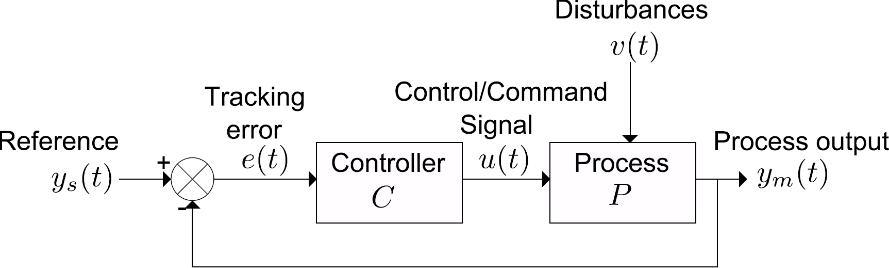
\includegraphics[width=.8\textwidth]{media/closed-loop.png}
\end{center}

where:
\begin{itemize}
    \item $y_s(t)$ is the desired or required process output (setpoint).
    \item $y(t)$ is the actual momentary output of the process. This signal is usually measured by a sensor.
    \item $e(t) = y_s(t) - y(t)$ is the tracking error.
    \item $u(t)$ is the input of the process (manipulated variable).
    \item $v(t)$ is the disturbance variable, which is an unwanted input to the process.
\end{itemize}

\section{Controllers}
\subsection{Disturbance rejection}
Disturbance rejection is the ability of a control system to minimize the impact of external
disturbances on the system’s output, ensuring that it remains as close as possible to the desired reference. The
disturbance rejection behavior quantifies how disturbances influence the process output, with a good disturbance
rejection behavior effectively minimizing these influences.

\subsubsection{Characteristics}
\begin{itemize}
    \item Disturbance types can be internal (e.g., component variations) or external (e.g., environmental changes)
    \item Effectiveness: a good controller detects and compensates for disturbances effectively
    \item Control strategies: feedback control (reactive) and feedforward control (proactive)
    \item Performance metrics:
    \begin{itemize}
        \item Stability: ensuring system robustness despite disturbances
        \item Steady-state error: minimizing deviation from the desired reference
        \item Overshoot/undershoot: controlling excessive deviations
        \item Rise time/settling time: ensuring fast and stable system response
    \end{itemize}
\end{itemize}

\subsection{Reference tracking}
Reference tracking behavior quantifies the deviation between the reference signal and the process
output (tracking error). A good reference tracking behavior minimizes this difference, ensuring the system follows
the desired reference as accurately as possible.

\subsubsection{Characteristics}
\begin{itemize}
    \item Tracking accuracy: the ability to follow the reference signal with minimal deviation
    \item Effectiveness: a good controller reduces tracking error across varying conditions
    \item Control strategies: feedback control (correcting deviations) and feedforward control (anticipating changes)
    \item Performance metrics:
    \begin{itemize}
        \item Stability: maintaining consistent tracking performance
        \item Steady-state error: minimizing long-term deviation from the reference
        \item Overshoot/undershoot: avoiding excessive deviations during tracking
        \item Rise time/settling time: achieving fast and stable convergence to the reference
    \end{itemize}
\end{itemize}

\subsection{Feedforward control}
Feedforward control is a predictive (proactive) control strategy that compensates for known internal
and external system influences before they affect the output. Unlike feedback control, which reacts to errors,
feedforward control anticipates changes and adjusts the system accordingly to improve performance.

\subsubsection{Reference feedforward}
\begin{itemize}
    \item Rapidly compensates for changes in the reference signal, before they impact the system
    \item Helps the system track the reference more accurately by preemptively adjusting the control input
    \item Example: If the desired sauna temperature (reference temperature) is increased from 70\cel to 90\cel, the heater’s power is immediately increased based on a precomputed model rather than waiting for feedback
\end{itemize}

\begin{center}
    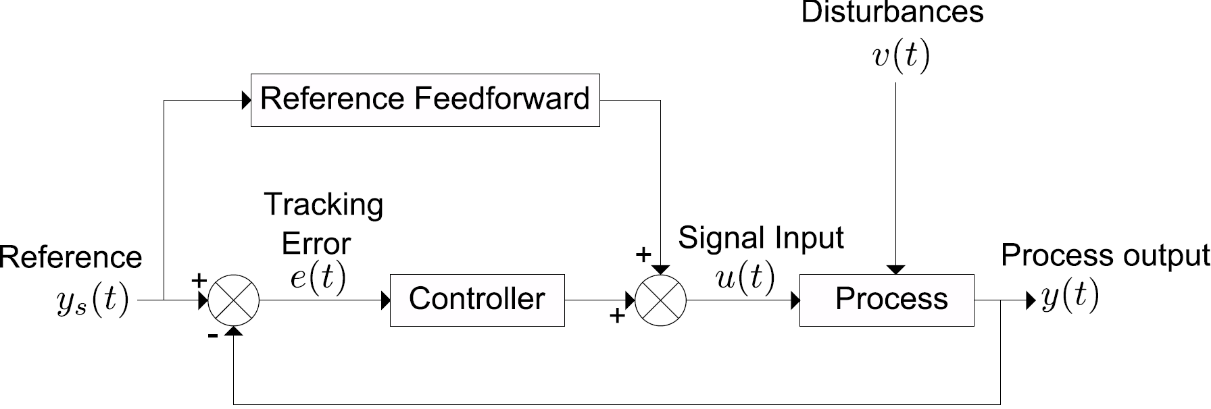
\includegraphics[width=\textwidth]{media/reference_feedforward.png}
\end{center}

\subsubsection{Disturbance feedforward}
\begin{itemize}
    \item Rapidly compensates for measurable disturbances, before they affect the process output
    \item Works by applying a precomputed correction based on the disturbance’s expected impact
    \item Example: If someone opens the sauna door, heat escapes, causing a potential drop in temperature. A feedforward controller detects the door opening and increases heating power preemptively to counteract the expected heat loss, reducing temperature fluctuations
\end{itemize}

\begin{center}
    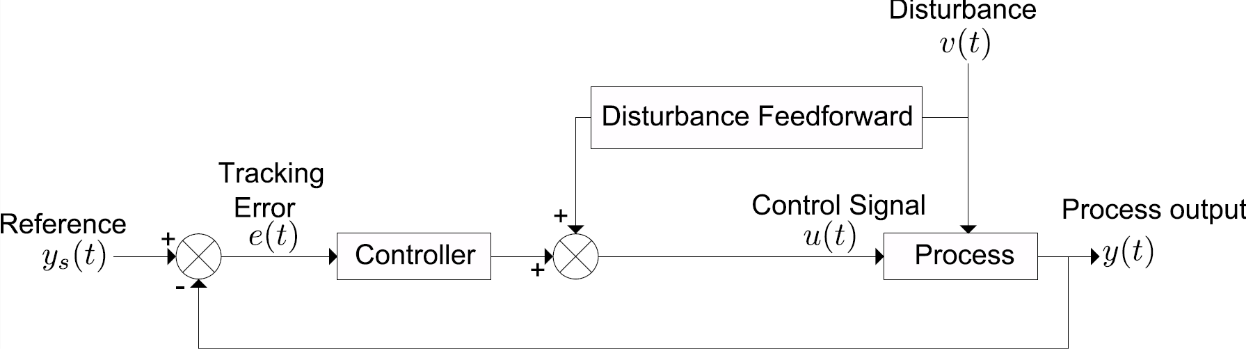
\includegraphics[width=\textwidth]{media/disturbance_feedforward.png}
\end{center}

\subsubsection{Reference and disturbance feedforward}
\begin{center}
    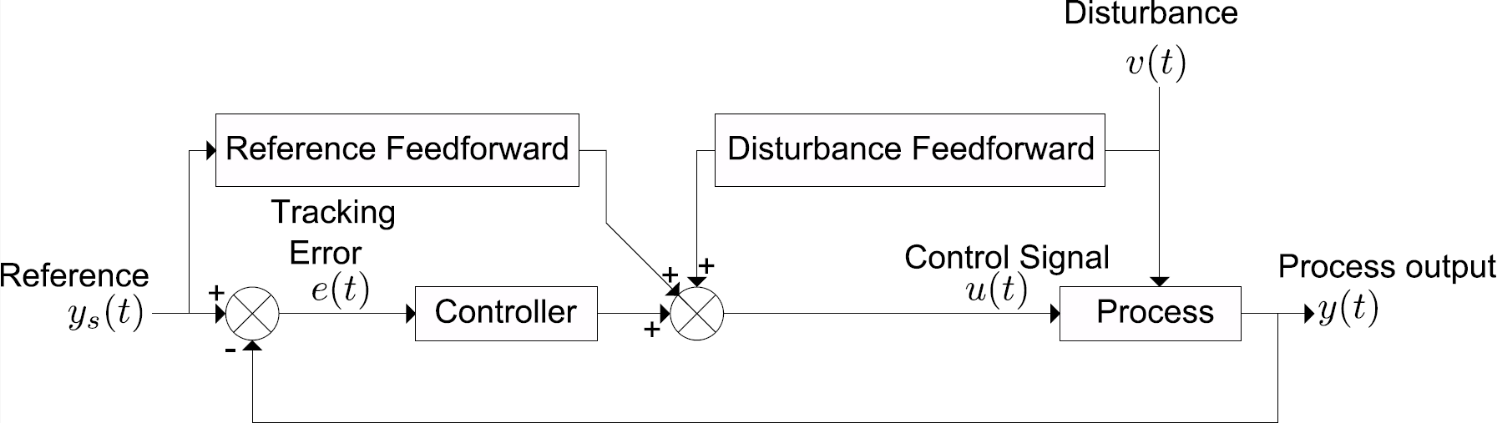
\includegraphics[width=\textwidth]{media/referencedisturbance_feedforward.png}
\end{center}

\section{Process model development}








\end{document}